\chapter{Evaluation}
\label{chapter:Evaluation}

The Evaluation will focus on the execution time of Jayvee pipelines, and how it has changed due to the optimizations described in previous chapters.

\section{Data source}
\label{section:data_source}

Jayvee pipelines require a data input with the following requirements

\subsection{Requirements}
%TODO: why not functional vs non-functional
\label{subsection:data_source_requirements}
\begin{description}
	\item[\ac{CSV} format] The dataset has to be available in a csv format, because the interpreter can only create tables from csv data.
	\item[openness] The dataset must have a licence conformant with the Open Definition \autocite{opendefinition}.
	      \textcite{opendefinition:licences} provides a list of recommended and conformant licenses.
\end{description}


\subsection{Chosen Dataset}
The selected dataset is entitled "Brewery Operations and Market Analysis" \autocite{dataset}.
The dataset does not contain real world data.
The dataset is licensed under the \ac{ODBbL}.
All data is contained in a single \ac{CSV} file, eliminating the need for table joins, which are not supported by Jayvee.

\subsubsection{Biases}
- dataset does not benefit any backend specifically %TODO

\section{Parameters}
\label{section:parameters}

The evaluation requires the execution of the Jayvee interpreter with different configurations.
A configuration is characterized by the enabled optimizations, the amount of transforms in the pipeline, and the number of rows in the input \ac{CSV} file.

We define the following optimization configurations.
\begin{description}
	%FIXME double enabled.
	\item[ts] TypeScript.
	      The baseline for the evaluateion.
	      It is intended to be as close as possible to the original implementation. %FIXME It is intended?
	\item[pl] Polars.
	      Enabled by starting the Jayvee interpreter with the \Verb|--use-polars| \ac{CLI} flag.
	      Enables the Polars implementations of tables, columns, block executors and transforms.
	\item[plob] Polars-One-Block.
	      Enabled by using the \Verb|LocalFileToTableExtractor| block (see \ref{arch:execs:localfiletotableextractor}) inside a pipeline and the \Verb|--use-polars| \ac{CLI} flag.
	      Enables pl, plus the \Verb|LocalFileToTableExtractor| block.
	\item[plrs] Polars-Rusqlite.
	      Enabled by the \Verb|--use-polars| and \Verb|--use-rusqlite| \ac{CLI} flags.
	      Enables pl, plus the \Verb|RustSQLiteLoaderExecutor| executor using the \Verb|sqlite-loader-lib| library.
	\item{plobrs} Polars-One-Block-Rusqlite.
	      Enabled by using the \Verb|LocalFileToTableExtractor| block and the \Verb|--use-polars| and \Verb|--use-rusqlite| \ac{CLI} flags.
	      Enables pl, plus \Verb|LocalFileToTableExtractor|, plus \Verb|RustSQLiteLoaderExecutor|.
\end{description}

We create three pipelines with the following amount of transforms
\begin{description}
	\item[none] The pipeline does not transform the data.
	\item[some] There are four transforms in the pipeline.
	\item[many] There are eight transforms in the pipeline.
\end{description}

We set six values for the amount of input rows: %FIXME: 1300000 is missing
$56250$, $112500$, $225000$, $4500000$, $900000$ ,$1800000$

A configuration picks one value from each category.


\section{The evaluation tool}
In order to automate the execution of the jayvee interpreter with the correct configurations, a \ac{CLI} program is created, the evaluation tool (see \ref{fig:uml:evalation-tool}).
The tool creates a list of all possible configurations and runs each of them 10 times, saving the execution duration.
It also uses \Verb|sqldiff| \ac{CLI} program \autocite{sqldiff}, to verify that the created databases are identical.
The timing of the execution duration includes code written by \textcite{so:benchmark}.

\begin{figure}
	\begin{plantuml}
		@startuml
		start
		while (For each combination of\nrowcount and amount of transforms)
		while (For each optimization)
		while (10 times)
		:start timer;
		:Run Jayvee interpreter with the configuration;
		:stop timer and save duration;
		endwhile
		:Calculate average and
		standard deviation;
		endwhile (done)
		if (sqldiff reports differences)
		:Print an error;
		endif
		endwhile (done)
		stop
		@enduml
	\end{plantuml}
	\caption{The evaluation tool's activity diagram}
	\label{fig:uml:evalation-tool}
\end{figure}

\subsection{Running a configuration}
This subsection outlines how the configuration is actually run.

It involves creating a source file with the correct amount of lines,
Selecting the correct Jayvee source file, and passing the location of the source and destination files as command line arguments.

The \Verb|head| \ac{CLI} program outputs the first lines of a file \autocite{head}.
Given that one line in the \ac{CSV} file represents one row of data, %TODO BE CERTAIN!
\mint{bash}{head --lines=<NUMBER_OF_ROWS> brewery_data_all.csv > l-<NUMBER_OF_ROWS>.csv}
generates a \ac{CSV} file with the requisite number of rows.

Given that there are three distinct numbers of transform amounts, three separate Jayvee source files are created.
For each of these, a variant incorporating the \Verb|LocalFileToTableExtractor| block is required, resulting in a total of six.
\ref{fig:uml:pick-jv-model} outlines the process by which the evaluation tool selects the correct source file.
\begin{figure}
	\begin{plantuml}
		@startuml
		!pragma useVerticalIf on
		start
		if (no transforms) then (yes)
		if (plob or plobrs enabled) then (yes)
		:plob-no.jv;
		stop
		else (ts, pl or plrs enabled)
		:ts-no.jv;
		stop
		endif
		elseif (some transforms) then
		if (plob or plobrs enabled) then (yes)
		:plob-so.jv;
		stop
		else (ts, pl or plrs enabled)
		:ts-so.jv;
		stop
		endif
		else (many transforms)
		if (plob or plobrs enabled) then (yes)
		:plob-ma.jv;
		stop
		else (ts, pl or plrs enabled)
		:ts-ma.jv;
		stop
		endif
		endif
		@enduml
	\end{plantuml}
	\caption{This diagram describes the process, by which the evaluation tool identifies the correct source file.}
	\label{fig:uml:pick-jv-model}
\end{figure}

The path of the \ac{CSV} data source, as well as the path of the destination database, are passed to the Jayvee interpreter via runtime parameters \autocite{jvalue:jayvee:docs:runtime}.

\ref{lst:run_config} outlines the whole process.

\begin{listing}
	\begin{minted}{python}
def run_config(interpreter_dir, rowcount, transforms, backend):
		source = f"l-{rowcount}.csv"
		run f"head --lines=${rowcount} brewery_data_all.csv > {source}"
		source_file = ... # Omitted the source file selection.
		destination = f"{backend}-{transforms}-{rowcount}.sqlite"

		command = f"node dist/apps/interpreter/main.js {source_file} -e SRC={source} -e SRC {destination}";

		if backend != "ts":
			command += " --use-polars"

		if backend == "plobrs" or backend == "plrs":
			command += " --use-rusqlite"

		start = now()
		execute(command)
		duration = now() - start
		return duration
	\end{minted}
	\caption{Pseudocode illustrating the manner in which the evaluation tool executes a configuration} %FIXME: is it pseudocode?
	\label{lst:run_config}
\end{listing}

\subsection{Evaluation Pipelines}

This subsection describes the Jayvee pipelines that get executed during the evaluation.

In total, there are six different pipelines, each with its own file.
The pipelines differ in two ways: how they extract the data from the data file and how many transforms are in the pipeline.
The former way is visualized in \ref{fig:uml:pipelines:backends},
the latter in \ref{fig:uml:pipelines:transforms}.
\begin{figure}
	\begin{subfigure}[h]{0.45\linewidth}
		\begin{plantuml}
			@startuml
			start
			-> None;
			::LocalFileExtractor;
			-> File;
			::TextFileInterpreter;
			-> TextFile;
			::CSVInterpreter;
			-> Sheet;
			::TableInterpreter;
			-> Table;
			stop
			@enduml
		\end{plantuml}
		\caption{ts}
		\label{fig:uml:pipelines:ts}
	\end{subfigure}
	\hfill
	\begin{subfigure}[h]{0.45\linewidth}
		\begin{plantuml}
			@startuml
			start
			-> None;
			::LocalFileToTableExtractor;
			-> Table;
			stop
			@enduml
		\end{plantuml}
		\caption{plobrs}
		\label{fig:uml:pipelines:plob}
	\end{subfigure}
	\caption{The initial section of Jayvee pipelines in Jayvee files starting with \dots . Presents the block's types and their associated IOType}
	\label{fig:uml:pipelines:backends}
\end{figure}

\begin{figure}
	\begin{subfigure}[h]{0.3\linewidth}
		\begin{plantuml}
			@startuml
			start
			-> Table;
			:LiquorLoader :SQLiteLoader;
			-> None;
			stop
			@enduml
		\end{plantuml}
		\caption{none}
	\end{subfigure}
	\hfill
	\begin{subfigure}[h]{0.3\linewidth}
		\begin{plantuml}
			@startuml
			start
			:AddColumnOne :TableTransformer;
			:BitPlusVol :TableTransformer;
			:UpdatePHLevel :TableTransformer;
			:SoldSqrt :TableTransformer;
			:LiquorLoader :SQLiteLoader;
			stop
			@enduml
		\end{plantuml}
		\caption{some}
	\end{subfigure}
	\hfill
	\begin{subfigure}[h]{0.3\linewidth}
		\begin{plantuml}
			@startuml
			start
			:AddColumnOne :TableTransformer;
			:BitPlusVol :TableTransformer;
			:UpdatePHLevel :TableTransformer;
			:SoldSqrt :TableTransformer;
			:AddColmumnOneDuplicate :TableTransformer;
			:BitPlusVolDuplicate :TableTransformer;
			:UpdatePHLevelDuplicate :TableTransformer;
			:SoldSqrtDuplicate :TableTransformer;
			:LiquorLoader: SQLiteLoader;
			stop
			@enduml
		\end{plantuml}
		\caption{many}
	\end{subfigure}
	\caption{How pipelines with \dots transform the input data.
		Displays block names and types.
	}
	\label{fig:uml:pipelines:transforms}
\end{figure}

\begin{description}
	\item[AddColumnOne] Adds a column filled with the value one.
	\item[BitPlusVol] Adds a column containing the sum of the columns "Bitterness" and "Volume\_Produced".
	\item[UpdatePHLevel] Multiplies the "ph\_Level" column by $10 000$.
	\item[SoldSqrt] Adds a column containing the square root values of the "Total Sales" column.
\end{description}

The implementation of string operations, such as \Verb|lowercase|, was not completed until after the conclusion of the evaluation process.
Consequently, the aforementioned pipelines do not contain such operations.

\section{Maximum Size of the input data}
During the evaluation process, we encountered Jayvee interpreter crashes.
We observed, that reducing the size of the input file appeared to prevent these crashes.
We subsequently narrowed down the exact limit to a range of $100 000$ lines, or $25\ac{MB}$.
This limit depends on the enabled optimizations and the amount of transforms in the pipeline.
\ref{tab:crashes} contains a table of maximum file sizes for each configuration and a snippet of the crash's error message.

Based on our knowledge of the interpreter, the "Invalid string lenght" error originates from a nodejs limit on the maximum length of a string. %FIXME make sure this is ok
The observation, that the error occurs during the loading of the table into the SQLite database, suggests, that the string limit may be exceeded during the generation of the \ac{SQL} queries.

The error message "JavaScript heap overflow", which also occurs is the \Verb|SQLiteLoader| block, indicates that the heap can not contain the data and the \ac{SQL} queries.

The error message "Cannot make a string longer than 0x1fffffe8 characters." is emitted, during the execution of a block with type \Verb|TextFileInterpreter|.

\begin{figure}
	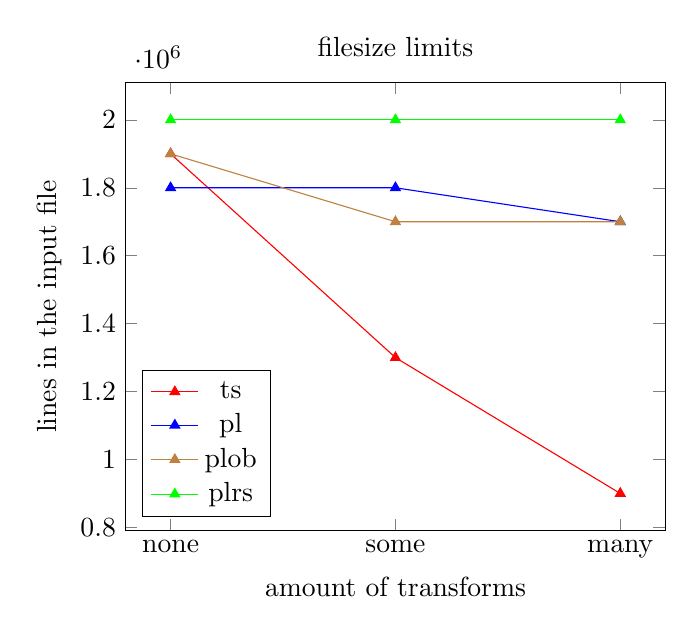
\begin{tikzpicture}
		\begin{axis}[
				title = {filesize limits},
				xlabel = {amount of transforms},
				ylabel = {lines in the input file},
				xtick = {1,2,3},
				xticklabels={none,some,many},
				legend pos=south west,
			]
			\addplot[
				color = red,
				mark=triangle*,
			]
			coordinates {
					(1,1900000)(2,1300000)(3,900000)
				};
			\addlegendentry{ts}
			\addplot[
				color=blue,
				mark=triangle*,
			]
			coordinates {
					(1,1800000)(2,1800000)(3,1700000)
				};
			\addlegendentry{pl}
			\addplot[
				color=brown,
				mark=triangle*,
			]
			coordinates {
					(1,1900000)(2,1700000)(3,1700000)
				};
			\addlegendentry{plob}
			\addplot[
				color=green,
				mark=triangle*,
			]
			coordinates {
					(1,2000000)(2,2000000)(3,2000000)
				};
			\addlegendentry{plrs}
		\end{axis}
	\end{tikzpicture}
	\caption{Maximum file sizes}
	\label{fig:plot:filesize}
\end{figure}

Considering these resuts, we conclude, that enabling optimizations increases the amount of data the Jayvee interpreter is able to process.


\section{the numbers}
\begin{figure}
	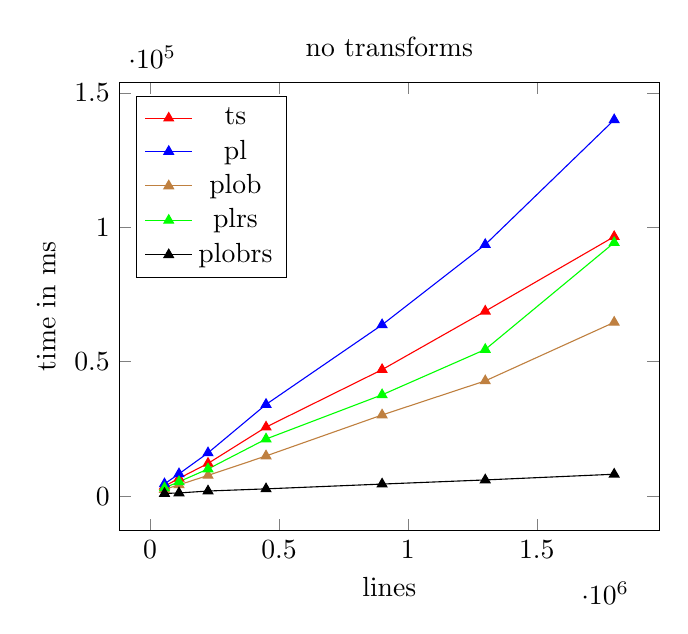
\begin{tikzpicture}
		\begin{axis}[
				title = {no transforms},
				% axis lines = left,
				xlabel = {lines},
				ylabel = {time in ms},
				% xtick={0,56250,112500,225000,450000,900000,1800000},
				legend pos=north west,
			]
			\addplot[
				color = red,
				mark=triangle*,
			]
			coordinates {
					(56250,3724)(112500,6648)(225000,12202)(450000,25701)(900000,47064)(1300000,68801)(1800000,96513)
				};
			\addplot[
				color=blue,
				mark=triangle*,
			]
			coordinates {
					(56250,4581)(112500,8323)(225000,16118)(450000,34125)(900000,63728)(1300000,93559)(1800000,139939)
				};
			\addplot[
				color=brown,
				mark=triangle*,
			]
			coordinates {
					(56250,2531)(112500,4231)(225000,7739)(450000,14976)(900000,30211)(1300000,42888)(1800000,64660)
				};
			\addplot[
				color=green,
				mark=triangle*,
			]
			coordinates {
					(56250,3102)(112500,5390)(225000,10126)(450000,21270)(900000,37705)(1300000,54562)(1800000,94274)
				};
			\addplot[
				mark=triangle*,
			]
			coordinates {
					(56250,1035)(112500,1221)(225000,1936)(450000,2740)(900000,4526)(1300000,6060)(1800000,8184)
				};

			\legend{ts,pl,plob,plrs,plobrs}
		\end{axis}
	\end{tikzpicture}
	\caption{plot no transforms}\label{fig:plot_no_transforms}
\end{figure}

\begin{figure}
	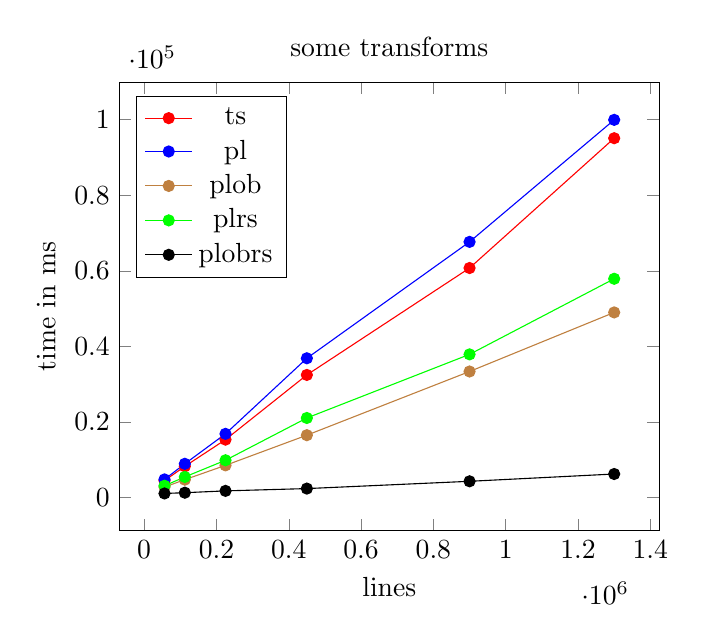
\begin{tikzpicture}
		\begin{axis}[
				title = {some transforms},
				% axis lines = left,
				xlabel = {lines},
				ylabel = {time in ms},
				% xtick={0,56250,112500,225000,450000,900000,1800000},
				legend pos=north west,
			]
			\addplot[
				color = red,
				mark=*,
			]
			coordinates {
					(56250,4495)(112500,8283)(225000,15346)(450000,32467)(900000,60755)(1300000,95102)
				};
			\addplot[
				color=blue,
				mark=*,
			]
			coordinates {
					(56250,4825)(112500,8952)(225000,16881)(450000,36874)(900000,67674)(1300000,99959)
				};
			\addplot[
				color=brown,
				mark=*,
			]
			coordinates {
					(56250,2804)(112500,4756)(225000,8544)(450000,16524)(900000,33375)(1300000,49007)
				};
			\addplot[
				color=green,
				mark=*,
			]
			coordinates {
					(56250,3144)(112500,5479)(225000,9894)(450000,21076)(900000,37910)(1300000,57910)
				};
			\addplot[
				mark=*,
			]
			coordinates {
					(56250,1106)(112500,1305)(225000,1789)(450000,2396)(900000,4323)(1300000,6252)
				};

			\legend{ts,pl,plob,plrs,plobrs}
		\end{axis}
	\end{tikzpicture}
	\caption{plot some transforms}\label{fig:plot_so_transforms}
\end{figure}

\begin{figure}
	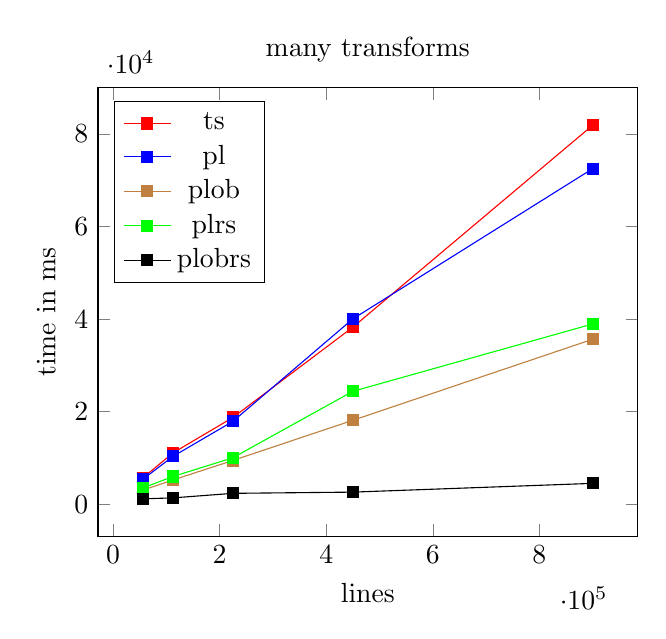
\begin{tikzpicture}
		\begin{axis}[
				title = {many transforms},
				% axis lines = left,
				xlabel = {lines},
				ylabel = {time in ms},
				% xtick={0,56250,112500,225000,450000,900000,1800000},
				legend pos=north west,
			]
			\addplot[
				color = red,
				mark=square*,
			]
			coordinates {
					(56250,5722)(112500,11097)(225000,18750)(450000,38264)(900000,81900)
				};
			\addplot[
				color=blue,
				mark=square*,
			]
			coordinates {

					(56250,5421)(112500,10348)(225000,17914)(450000,40054)(900000,72515)

				};
			\addplot[
				color=brown,
				mark=square*,
			]
			coordinates {

					(56250,3064)(112500,5248)(225000,9470)(450000,18147)(900000,35656)

				};
			\addplot[
				color=green,
				mark=square*,
			]
			coordinates {
					(56250,3545)(112500,5997)(225000,10051)(450000,24406)(900000,38963)
				};
			\addplot[
				mark=square*,
			]
			coordinates {
					(56250,1178)(112500,1383)(225000,2365)(450000,2627)(900000,4518)
				};

			\legend{ts,pl,plob,plrs,plobrs}
		\end{axis}
	\end{tikzpicture}
	\caption{plot many transforms}\label{fig:plot_ma_transforms}
\end{figure}

\begin{figure}
	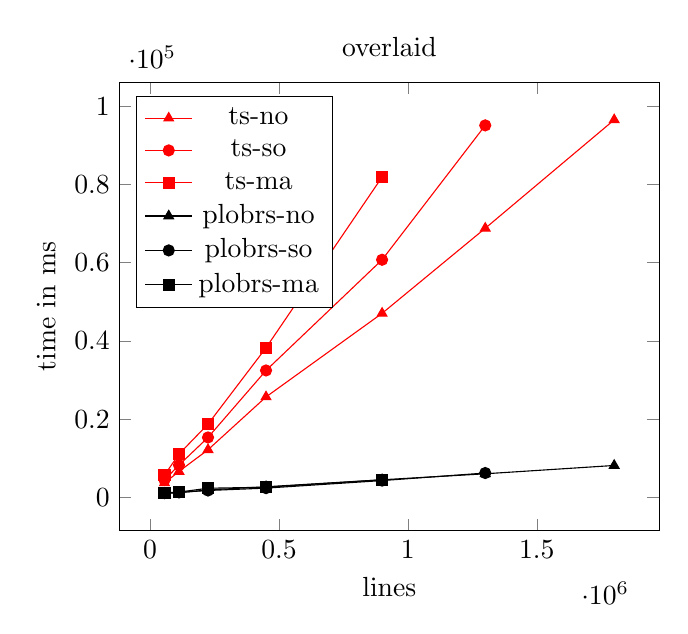
\begin{tikzpicture}
		\begin{axis}[
				title = {overlaid},
				% axis lines = left,
				xlabel = {lines},
				ylabel = {time in ms},
				% xtick={0,56250,112500,225000,450000,900000,1800000},
				legend pos=north west,
			]
			\addplot[
				color = red,
				mark=triangle*,
			]
			coordinates {
					(56250,3724)(112500,6648)(225000,12202)(450000,25701)(900000,47064)(1300000,68801)(1800000,96513)
				};
			\addlegendentry{ts-no}
			\addplot[
				color = red,
				mark=*,
			]
			coordinates {
					(56250,4495)(112500,8283)(225000,15346)(450000,32467)(900000,60755)(1300000,95102)
				};
			\addlegendentry{ts-so}
			\addplot[
				color = red,
				mark=square*,
			]
			coordinates {
					(56250,5722)(112500,11097)(225000,18750)(450000,38264)(900000,81900)
				};
			\addlegendentry{ts-ma}
			\addplot[
				mark=triangle*,
			]
			coordinates {
					(56250,1035)(112500,1221)(225000,1936)(450000,2740)(900000,4526)(1300000,6060)(1800000,8184)
				};
			\addlegendentry{plobrs-no}
			\addplot[
				mark=*,
			]
			coordinates {
					(56250,1106)(112500,1305)(225000,1789)(450000,2396)(900000,4323)(1300000,6252)
				};
			\addlegendentry{plobrs-so}
			\addplot[
				mark=square*,
			]
			coordinates {
					(56250,1178)(112500,1383)(225000,2365)(450000,2627)(900000,4518)
				};
			\addlegendentry{plobrs-ma}
		\end{axis}
	\end{tikzpicture}
	\caption{plot transforms}\label{fig:plot:ts_vs_plobrs}
\end{figure}

\begin{figure}
	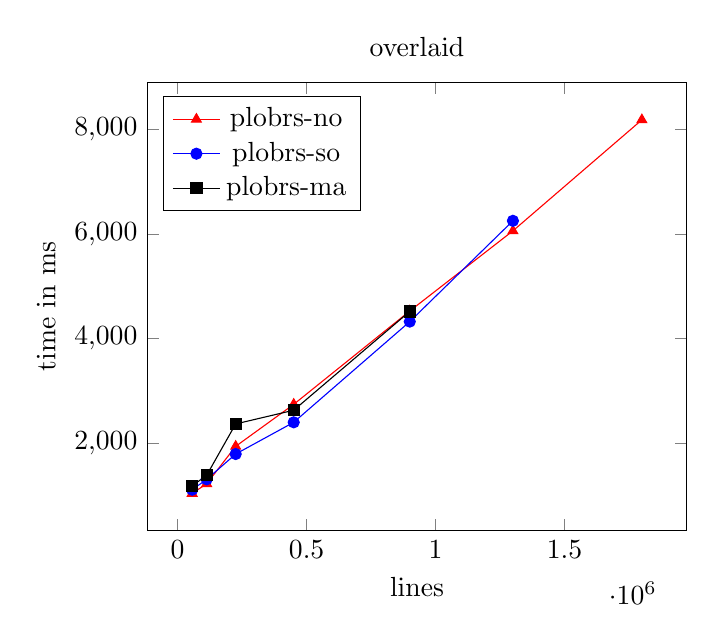
\begin{tikzpicture}
		\begin{axis}[
				title = {overlaid},
				% axis lines = left,
				xlabel = {lines},
				ylabel = {time in ms},
				% xtick={0,56250,112500,225000,450000,900000,1800000},
				legend pos=north west,
			]
			\addplot[
				color = red,
				mark=triangle*,
			]
			coordinates {
					(56250,1035)(112500,1221)(225000,1936)(450000,2740)(900000,4526)(1300000,6060)(1800000,8184)
				};
			\addlegendentry{plobrs-no}
			\addplot[
				color = blue,
				mark=*,
			]
			coordinates {
					(56250,1106)(112500,1305)(225000,1789)(450000,2396)(900000,4323)(1300000,6252)
				};
			\addlegendentry{plobrs-so}
			\addplot[
				mark=square*,
			]
			coordinates {
					(56250,1178)(112500,1383)(225000,2365)(450000,2627)(900000,4518)
				};
			\addlegendentry{plobrs-ma}
		\end{axis}
	\end{tikzpicture}
	\caption{plot transforms}\label{fig:plot:plobrs}
\end{figure}



\subsection{no transforms vs some transforms vs many transforms}
\subsubsection{no transforms}
- pl is slowest, because:
- no transforms yet, so no speedup from there
- from comparing the debug output of two example runs we can see that PolarsSQLiteLoaderExecutor is slower than TsSQLiteLoaderExecutor %TODO: provide numbers
- the one block optimization yields better results than the rust sqlite loader implementation
- plobrs is the best

\subsubsection{some transforms}
- ts is still better than pl but it' close now
- same the introduction of transforms made it closer
- prediction: many transforms will make pl faster
- other than that the same result

\subsubsection{many transforms}
- trend continues, now pl is faster, except once
- the rest remains the same

- TODO: adding transforms increased the runtime by a factor of x

\subsection{ts vs plobrs}
- calculate ts \/ plobrs
- see table
- the more lines, the bigger the ingrease for plobrs,
- the more transforms, the bigger the advantage for plobrs

\begin{figure}
	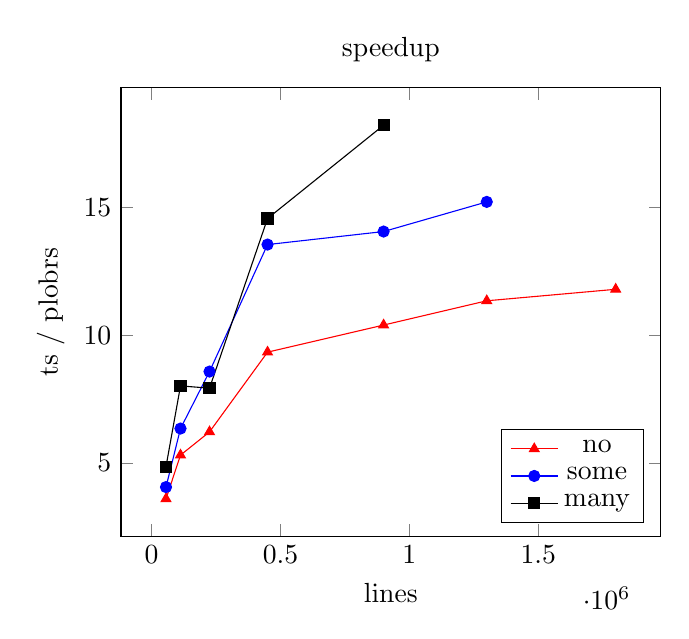
\begin{tikzpicture}
		\begin{axis}[
				title = {speedup},
				% axis lines = left,
				xlabel = {lines},
				ylabel = {ts / plobrs},
				legend pos=south east,
			]
			\addplot[
				color = red,
				mark=triangle*,
			]
			coordinates {
					(56250,3.60)(112500,5.31)(225000,6.22)(450000,9.34)(900000,10.40)(1300000,11.35)(1800000,11.80)
				};
			\addlegendentry{no}
			\addplot[
				color = blue,
				mark=*,
			]
			coordinates {
					(56250,4.06)(112500,6.35)(225000,8.58)(450000,13.55)(900000,14.06)(1300000,15.22)
				};
			\addlegendentry{some}
			\addplot[
				mark=square*,
			]
			coordinates {
					(56250,4.86)(112500,8.02)(225000,7.93)(450000,14.57)(900000,18.22)
				};
			\addlegendentry{many}
		\end{axis}
	\end{tikzpicture}
	\caption{speedup factors}\label{fig:plot:factor}
\end{figure}








\section{Reevaluating the requirements}
\subsection{FR}
- interop DONE, because sqlite library and shows interop
- coloumnar DONE, because polars is build on apache arrow
- compatibility DONE, vehicles works, but: some operators that arent used in vehicles arent supported, but could be with more time, or without the compatibility requirement
- null is in the polars tables, can be removed with more work.
- some floats are slightly different (EXAMPLE!). maybe because of different widths?
- modularization ALMOST, the rust stuff is in a sperate library, but that library is outside of the monorepo

\subsection{NFR}
- performance DONE, see evaluation above
- readability IDK, readabyility might not be the correct term here.
the code is understandable for non-rust people (except sqlite-loader-lib).
- codestyle DONE, only eslint errors are from testing files, which are excluded because prototype.
clippy and rustfmt doesnt have suggestions for rust code.
- maturity DONE maybe dont mention this as a requirement.
- extensibility DONE, we wrote sqlite-loader-lib, which exports polars tables to sqlite, polars doesnt support this ootb.
